\chapter{Overall results and evaluation}
\label{chapter:overall-results}

\todo{TODO: Results and evaluation; tables; images; \ldots}\\
\todo{Obrázky obou postprocessoru (desktop, web-based), různé filtry - řezy, isoplochy (temelin a karluv most bude vypadat pekne (chotkova a shear beam uz jsou pouzity v predchozich kapitolach)).}\\
\todo{Zmerit latenci - pocatecni delay, pred zobrazenim site/dat. Zmerit pocet snimku za sekundu. Porovnat napr s tradicnim postprocesorem a pak se Simscale? Zmerit pametovou narocnost puvodniho a noveho postprocesoru (porovnat s GiDem jako s tradicnim postprocesorem).}\\
\todo{Vysvetlit, proc jsem navrhl tyto testy a benchmarky. Co se snazim dokazat? Snazim se ospravedlnit vyvoj noveho formatu a kompresni metody...}\\


\begin{figure}[H]
    \centering
    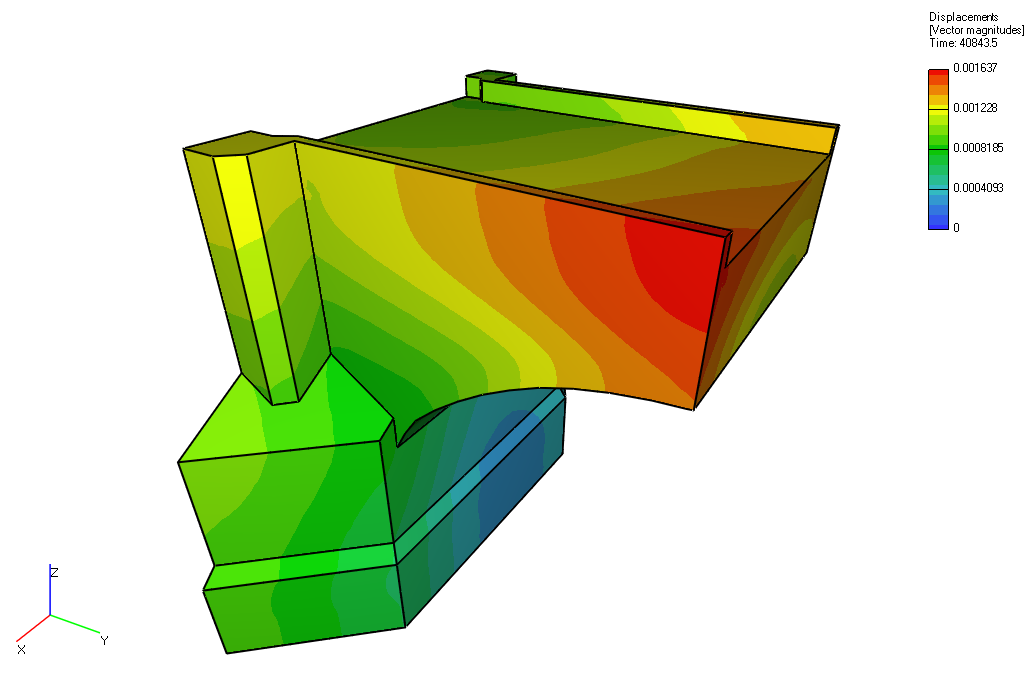
\includegraphics[width=\textwidth]{figures/chapter-results/charles-bridge-model}
    \decoRule
    \caption[Model of Charles Bridge in Prague -- heat transport analysis results]{Model of Charles Bridge in Prague: heat transport analysis results (displacements).}
    \label{fig:charles-bridge-model}
  \end{figure}

\begin{figure}[H]
  \centering
  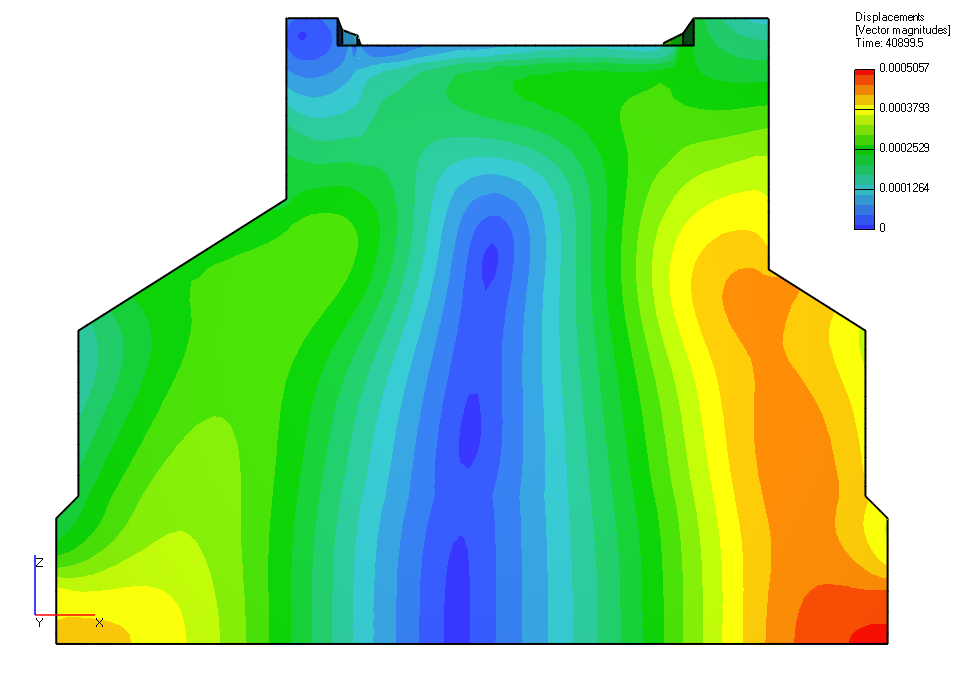
\includegraphics[width=\textwidth]{figures/chapter-results/charles-bridge-exact-data-values}
  \decoRule
  \caption[Model of Charles Bridge -- exact data values]{Model of Charles Bridge in Prague: exact data values of heat transport analysis results, no approximation applied.}
  \label{fig:charles-bridge-exact-data-values}
\end{figure}

\begin{figure}[H]
  \centering
  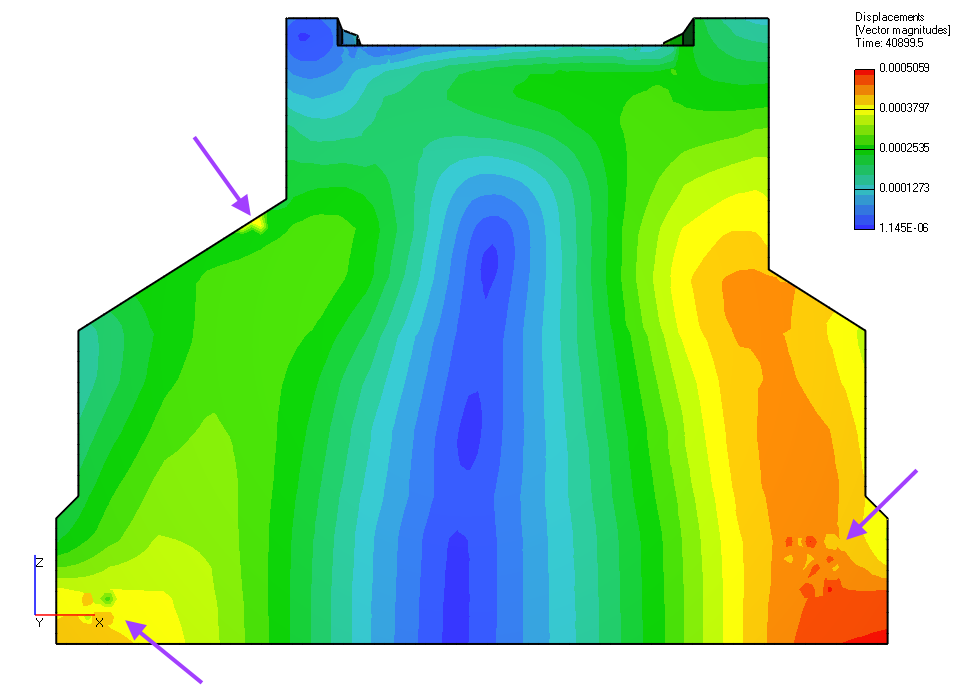
\includegraphics[width=\textwidth]{figures/chapter-results/charles-bridge-approximation-method-artifacts}
  \decoRule
  \caption[Model of Charles Bridge -- approximation method's artifacts]{Model of Charles Bridge in Prague: heat transport analysis results, approximation method's artifacts (marked by arrows).}
  \label{fig:charles-bridge-approximation-method-artifacts}
\end{figure}

\begin{figure}[H]
  \centering
  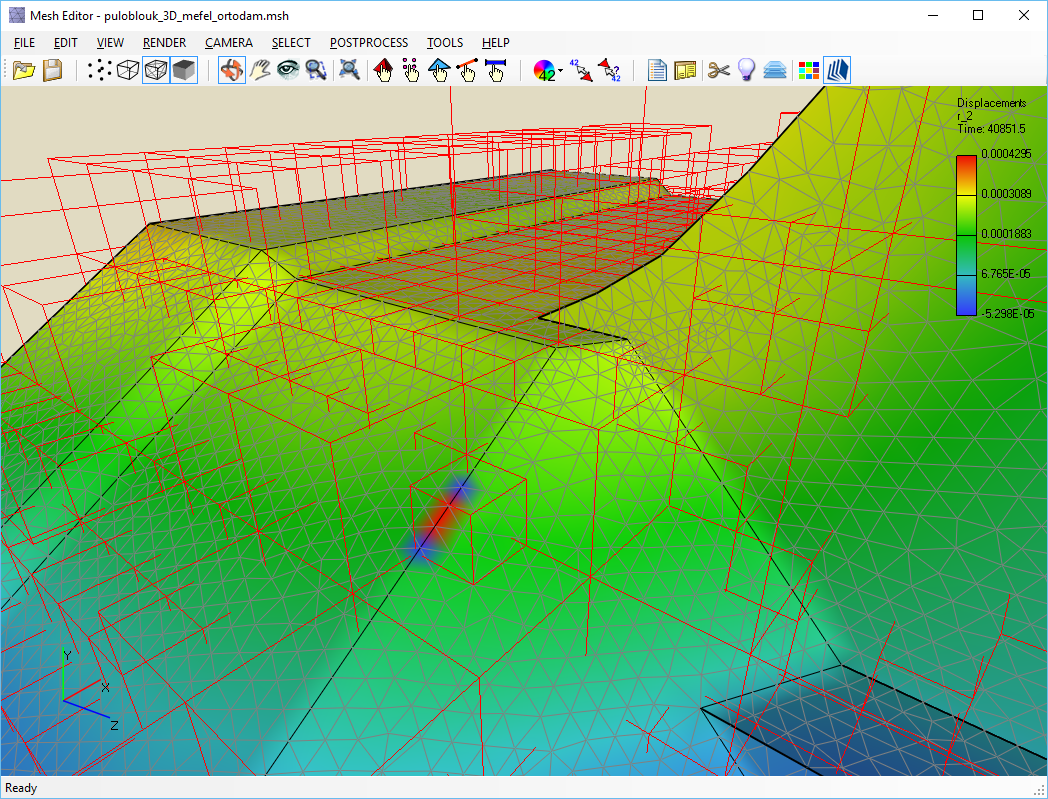
\includegraphics[width=\textwidth]{figures/chapter-results/charles-bridge-glitches-in-approximation}
  \decoRule
  \caption[Model of Charles Bridge -- glitches in approximation function]{Model of Charles Bridge in Prague: glitches in approximation function caused by octree-based space decomposition. The red lines represent the octree segments.}
  \label{fig:charles-bridge-glitches-in-approximation}
\end{figure}
